% rubber: module biber
\documentclass[xcolor=pst]{beamer}
\usepackage[utf8]{inputenc}
\usepackage{ngerman}
\usepackage{beamerthemesplit}
\usepackage{epsfig}
\usepackage{tikz}
\usepackage{siunitx}
\usepackage{pbox}
\usepackage{pdfpages}
\usepackage{verbatim}
\usepackage{units}
\usepackage{algpseudocode}

\usepackage{color}
\usetheme{Antibes}
%\usepackage{multirow}

% an seitenbreite angepasste tabellen
\usepackage{booktabs}
\usepackage{tabularx} % page-width
\usepackage{adjustbox}

% tabulatoren in itemize
\usepackage{tabto}

% bibliographie
\usepackage[english]{cleveref}
\usepackage[style=authoryear-comp,backend=biber]{biblatex}
\addbibresource{literatur.bib}
\usepackage{appendixnumberbeamer}

\usetikzlibrary{shapes.geometric, positioning, calc, shapes, fit, backgrounds}

% fusszeile so aufteilen, dass autoren und titel reinpassen und seitenzahl hinzu
\setbeamertemplate{footline}
{
  \leavevmode%
  \hbox{%
  \begin{beamercolorbox}[wd=.6\paperwidth,ht=2.25ex,dp=1ex,center]{author in head/foot}%
    \usebeamerfont{author in head/foot}\insertshortauthor
  \end{beamercolorbox}%
  \begin{beamercolorbox}[wd=.4\paperwidth,ht=2.25ex,dp=1ex,center]{title in head/foot}%
    \usebeamerfont{title in head/foot}\insertshorttitle\hspace*{2.5em}\insertframenumber
  \end{beamercolorbox}}%
  \vskip0pt%
}

% keine navigationssymbole in der fusszeile
\beamertemplatenavigationsymbolsempty

% so definiert man neue makros
\newcommand{\IFF}{\Leftrightarrow}
\newcommand{\todo}[1]{\textbf{\color{red}todo:\color{black}#1}}

\author{
  Lukas Götz, Stefan Dang \& Dorle Osterode
}
\title{gt Scaffold}
\institute[]{}
\date{2015-01-30}

\subject{}
\keywords{}

\begin{document}
\begin{frame}[plain]
  \titlepage
\end{frame}

% keine seitenzahl auf der inhaltsangabe zeigen (theme nur fuer diese folie anpassen)
\bgroup
\makeatletter
\setbeamertemplate{footline}
{
  \leavevmode%
  \hbox{%
  \begin{beamercolorbox}[wd=.6\paperwidth,ht=2.25ex,dp=1ex,center]{author in head/foot}%
    \usebeamerfont{author in head/foot}\insertshortauthor
  \end{beamercolorbox}%
  \begin{beamercolorbox}[wd=.4\paperwidth,ht=2.25ex,dp=1ex,center]{title in head/foot}%
    \usebeamerfont{title in head/foot}\insertshorttitle\hspace*{2.5em}
  \end{beamercolorbox}}%
  \vskip0pt%
}
\makeatother
\begin{frame}{Übersicht}
  \tableofcontents
\end{frame}
\egroup % ab hier das normale theme weiterverwenden


\section{Motivation}
\subsection{Scaffolding}
\begin{frame}
\setcounter{framenumber}{1}
  \frametitle{Einführung}

  \begin{columns}
    \begin{column}{.45\textwidth}
      \begin{itemize}
      \item Assemblierung $\rightarrow$ Mehrere unabhängige Contigs
      \begin{itemize}
        \item Ungleichmäßige Coverage
        \item Wiederholungen
      \end{itemize}
      \item Motivation: Anordnung der Contigs in Scaffolds
      \begin{itemize}
        \item Richtung und relative Anordnung
        \item Paarweiser Abstand
      \end{itemize}
      \end{itemize}
    \end{column}
    \begin{column}{.45\textwidth}
      \begin{center}
        \begin{figure}[t]
          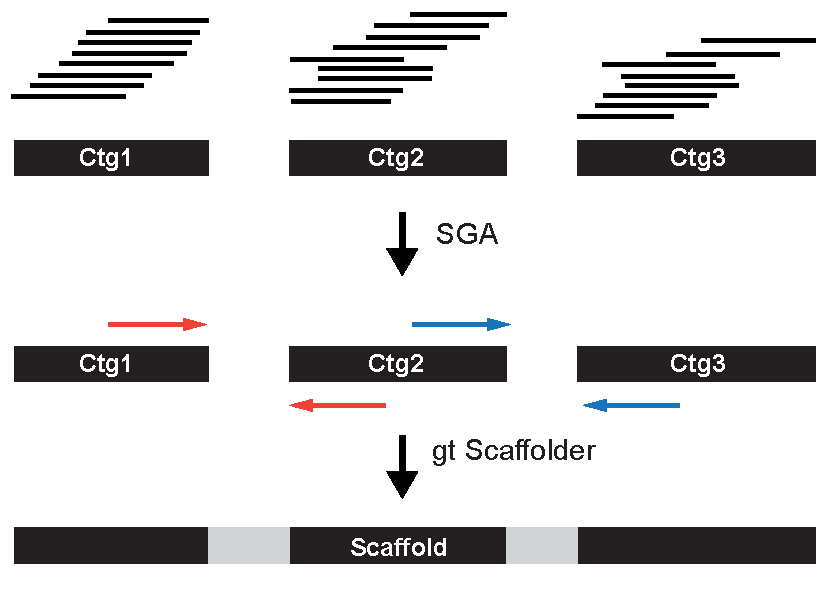
\includegraphics[width=\textwidth,height=0.8\textheight,keepaspectratio]{figures/Scaffolding.pdf}
        \end{figure}
        % SK: Paired-end erwähnen, siehe naechste Folie
      \end{center}
    \end{column}
  \end{columns}
\end{frame}

\begin{frame}
  \frametitle{Einführung}
  \begin{itemize}
  \item Verwendung der Read-Paar Informationen:
    \begin{itemize}
    \item Fragmentgröße
    \item Position auf Contigs
    \end{itemize}
  \item Read-Paare stammen aus paired-end oder mate-pair Sequenzierung
  \end{itemize}
\end{frame}

\begin{frame}
  \frametitle{Scaffolding Problem}
  \begin{itemize}
  \item Scaffold Graph:
    \begin{itemize}
    \item Knoten entsprechen Contigs
    \item Kanten beschreiben Read-Paar
      Informationen
    \item bidirektionaler Graph
    \end{itemize}
  \item Scaffolding ist NP-vollständig\footnote{\cite{Huson:2002kf}}
  \item Strategie: Zerlegung in % SK: Erweitern oder Weglassen
    Teilprobleme, die unabhängig voneinander gelöst werden
  %% \item Beschreibung des Scaffolding Problems mit Hilfe eines
  %%   Graphen (Scaffold Graph), wobei deren Zusammenhangskomponenten
  %%   Teilprobleme darstellen
  \end{itemize}
\end{frame}

\begin{frame}
  \frametitle{Scaffolding Problem}
  \begin{center}
    \includegraphics[width=\textwidth,height=\textheight,keepaspectratio]{figures/Scaffolding_graph.png}
  \end{center}
\end{frame}

\begin{frame}
  \frametitle{Ziel des Projektes}
  \begin{itemize}
  \item Entwicklung einer Scaffolding-Software und ihre Evaluierung
  \begin{itemize}
    \item Basierend auf Konzepten und Infrastruktur der \textit{GenomeTools}-Bibliothek\footnote{\cite{Gremme:2013}}
    \item Aufbauend auf Assemblierungs-Software \textit{Readjoiner}\footnote{\cite{Gonnella:2012gn}}
  \end{itemize}
  \item Methodische Anlehnung an \textit{SGA (String Graph Assembler)}\footnote{\cite{Simpson:2012ef}}
  \item Strategie von SGA-SCaffold
  \begin{itemize}
    \item Vereinfachung und Partitionierung eines Scaffold-Graphen
    \item Berechnung des Scaffolds als Pfad mit max. Sequenzabdeckung
  \end{itemize}
  \end{itemize}
\end{frame}

\section{Methoden}
% \begin{frame}
%   \frametitle{Allgemein}
%   \begin{itemize}
%   \item Reimplementation der Scaffolding Methode von SGA (C++) im
%     Rahmen von Genometools (C)
%   \item basiert auf Konstruktion eines Graphen über die Beziehungen
%     zwischen Contigs (Scaffold Graph)
%   \end{itemize}
% \end{frame}

\begin{frame}
  \frametitle{Übersicht der Schritte}

  \begin{tikzpicture}[every node/.style={font=\footnotesize}]
    \node[] (input1) {Contigs};
    \node[left of=input1, xshift=-1cm] (eingabe) {Eingabe:};
    \node[below of=eingabe, yshift=-5cm] (ausgabe) {Ausgabe:};
    \node[right of=input1, align=center, xshift=2cm] (input2) {Distanz-\\informationen};
    \node[right of=input2, xshift=2cm] (input3) {A-Statistik};

    \node[below of=input1, yshift=-.5cm, anchor=west] (titel) {gt Scaffolder};
    \node[rectangle, draw, anchor=west, below of=titel, xshift=1cm, rounded corners, fill=black!10, yshift=.25cm] (konstruktion) {Konstruktion des Graphen};
    \node[rectangle, draw, anchor=west, below of=konstruktion, xshift=.95cm, rounded corners, fill=black!10, yshift=.25cm] (selektion) {Selektion relevanter Knoten und Kanten};
    \node[rectangle, draw, anchor=west, below of=selektion, xshift=-1.35cm, rounded corners, fill=black!10, yshift=.25cm] (ermittlung) {Ermittlung aller ZKs};
    \node[rectangle, draw, anchor=west, below of=ermittlung, xshift=1.55cm, rounded corners, fill=black!10, yshift=.25cm] (pfade) {Bestimmung des besten Pfades für jede ZK};

    \begin{pgfonlayer}{background}
    \node[draw, fit={(titel) (konstruktion) (selektion) (ermittlung) (pfade)}, rounded corners, fill=black!20] (back) {};
    \end{pgfonlayer}

    \node[below of=back, yshift=-2cm, xshift=-1.5cm] (output1) {Scaffolds};
    \node[right of=output1, align=center, xshift=2cm, yshift=-.25cm] (output2) {(rekonstruierte\\Sequenzen)};
    \node[above of=output1] (dummy) {};

    \path[->, thick]
    (input1) edge (back)
    (input2) edge (back)
    (input3) edge (back)
    (back) edge (output1)
    (back) edge (output2);
  \end{tikzpicture}
\end{frame}

\begin{frame}
  \frametitle{Details der Schritte}
  TODO:\ Illustrieren der einzelnen Schritte
\end{frame}

\section{Ergebnisse}

\begin{frame} % SK: Gegenüberstlellung einfügen
  \frametitle{Erstellung Testdaten}
  \begin{itemize}
    \item Referenzsequenzen
    \begin{itemize}
      \item \textit{S. cerevisiae}       \tabto{3.5cm}~~12 Mbp \tabto{5cm} Ensembl R64-1-1
      \item \textit{H. sapiens}, Chr. 21 \tabto{3.5cm}~~48 Mbp \tabto{5cm} Ensembl GRCh37
      \item \textit{C. elegans}          \tabto{3.5cm}100 Mbp \tabto{5cm} Ensembl WBcel235
      \item \textit{D. melanogaster}     \tabto{3.5cm}140 Mbp \tabto{5cm} Ensembl BDGP5
    \end{itemize}
    \item Simulierte Paired-End-Reads durch \textit{art\_illumina}\footnote{\cite{Huang:2012kq}}
    \begin{itemize}
      \item Read-Länge 150 bp
      \item Coverage 20X
      \item Fragmentlänge 400 bp $\pm$ 10 bp
    \end{itemize}
    \item Assemblierung der Reads durch SGA-Pipeline
    \item TODO:\ Hardware einfügen (CPU, RAM, OS, bit)
  \end{itemize}
\end{frame}



\begin{frame}
  \frametitle{gt Scaffold vs. SGA Scaffold}
  \begin{table}
      \adjustbox{max height=\dimexpr\textheight-5.5cm\relax, max width=\textwidth}{
      \begin{tabular}{llccccc}
          \toprule
          Dataset & Program name & Total span (Mbp) & \#Scaffolds & $N50$ (kb) & CPU (s) & Mem (MB) \\
          \midrule
          \textit{S. cerevisiae}
                  & SGA Scaffold & 11.08            &       600   &  32.3   & 0.01      &  28.9 \\
                  & gt Scaffold  &                  &       600   &         & $1\times$ &  $0.43\times$ \\
          \midrule
          \textit{H. sapiens}, Chr. 21
                  & SGA Scaffold & 34.25            &      1368   &  54.2   & 0.04  &  27.8  \\
                  & gt Scaffold  &                  &      1368   &         & $1\times$ & $0.6\times$       \\
          \midrule
          \textit{C. elegans}
                  & SGA Scaffold & 94.07            &      5659   &  36.9   & 0.11  &  34.9 \\
                  & gt Scaffold  &                  &      5659   &         & $0.9\times$ & $0.90\times$      \\
          \midrule
          \textit{D. melanogaster}
                  & SGA Scaffold & 113.48           &      2281   &  126.3  & 0.11  & 29.2     \\
                  & gt Scaffold  &                  &      2281   &         & $0.9\times$ & $0.62\times$     \\
          \bottomrule
      \end{tabular}}
  \end{table}
\end{frame}

\begin{frame}
  \frametitle{Plot: gt Scaffold vs. SGA Scaffold}
  \begin{figure}[t]
    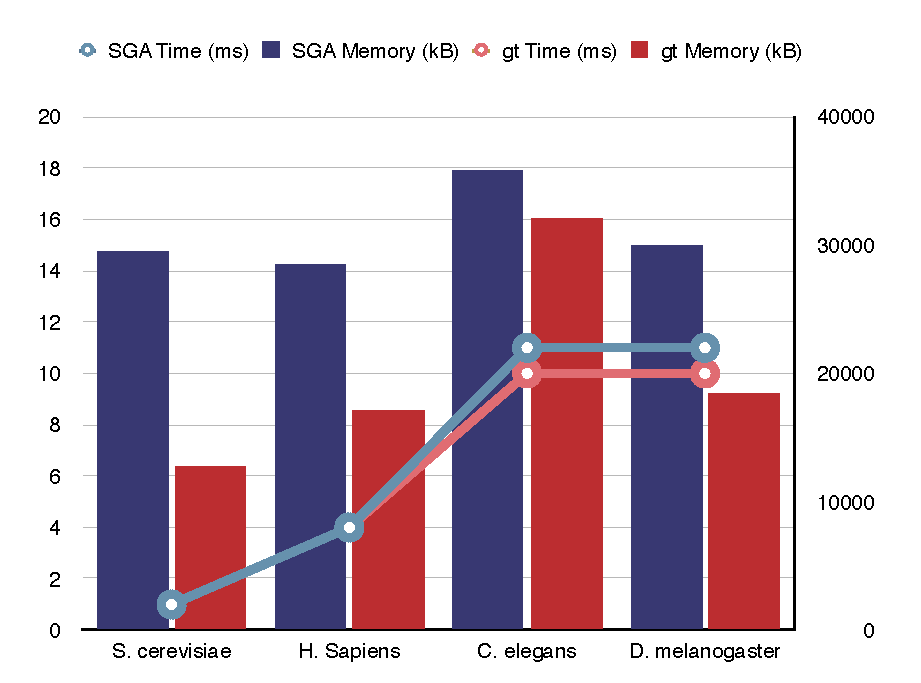
\includegraphics[width=\textwidth,height=0.8\textheight,keepaspectratio]{figures/sga_vs_gt.pdf}
  \end{figure}
\end{frame}

\section{Diskussion und Ausblick}
\begin{frame}
  \frametitle{Diskussion}
  \begin{itemize}
  \item Gründe für neue Implementation
    \begin{itemize}
    \item geringerer Speicherplatzverbrauch, aehnliche Laufzeit
       für gt Scaffold im Vergleich zu SGA Scaffold bei gleicher Güte
       der Ergebnisse
    \item keine externen Software-Abhängigkeiten
      %% A-Statistik: Python-Skript auf Basis von Pysam
      %% Distanz-Informationen: Fixmate, DistEst von Abyss, Samtools
    \end{itemize}
  \end{itemize}
  \begin{tikzpicture}[node distance=.75cm]
    \tikzstyle{prog}=[draw, rectangle, rounded corners, font=\tiny, rotate=90];
    \node[prog] (prep) {preprocess};
    \node[prog, below of=prep] (index) {index};
    \node[prog, below of=index] (correct) {correct};
    \node[prog, below of=correct] (index2) {index};
    \node[prog, below of=index2] (filter) {filter};
    \node[prog, below of=filter] (overlap) {overlap};
    \node[prog, below of=overlap] (assemble) {assemble};
    \node[prog, below of=assemble, fill=red!40] (bindex) {index};
    \node[prog, below of=bindex, fill=red!40] (aln) {align};
    \node[prog, below of=aln, fill=red!40] (sampe) {sampe};
    \node[prog, below of=sampe, rectangle split, rectangle split parts=3, yshift=-.45cm, rectangle split part fill={blue!40, green!40, blue!40}] (bam2de) {\nodepart{one}fixmate\nodepart{two}samtools\nodepart{three}DistanceEst};
    \node[prog, below of=bam2de, yshift=-.45cm, fill=yellow!40] (pysam) {astat};
    \node[prog, below of=pysam] (scaff) {scaffold};
    \node[prog, below of=scaff] (scaf2fasta) {scaf2fasta};

    \path[->]
    (prep) edge (index)
    (index) edge (correct)
    (correct) edge (index2)
    (index2) edge (filter)
    (filter) edge (overlap)
    (overlap) edge (assemble)
    (assemble) edge (bindex)
    (bindex) edge (aln)
    (aln) edge (sampe)
    (sampe) edge (bam2de)
    (bam2de) edge (pysam)
    (pysam) edge (scaff)
    (scaff) edge (scaf2fasta);
  \end{tikzpicture}

  \begin{tikzpicture}[node distance=.75cm]
    \tikzstyle{prog}=[draw, rectangle, rounded corners, font=\tiny, rotate=90];
    \node[prog] (prefilter) {prefilter};
    \node[prog, below of=prefilter] (overlap) {overlap};
    \node[prog, below of=overlap] (assembly) {assembly};
    \node[prog, below of=assembly] (scaffold) {scaffold};

    \path[->]
    (prefilter) edge (overlap)
    (overlap) edge (assembly)
    (assembly) edge (scaffold);
  \end{tikzpicture}
\end{frame}

\begin{frame}
  \frametitle{Ausblick}
  \begin{itemize}
  \item was wir noch alles machen muessen (kann erst am ende
    ausgefuellt werden)
  \end{itemize}
\end{frame}

\end{document}
